% !TeX program = xelatex
% MARKOU DESIGN LONDON — DIGITAL EXPERIENCE & CLIENT STUDY
% Compile with XeLaTeX (recommended) or LuaLaTeX.
\documentclass[10.5pt,a4paper]{article}

\usepackage[a4paper,top=20mm,bottom=22mm,left=20mm,right=20mm]{geometry}
\usepackage{fontspec}
\usepackage[english]{babel}
\usepackage{xcolor}
\usepackage{tikz}
\usetikzlibrary{calc,positioning}
\usepackage[most]{tcolorbox}
\usepackage{graphicx}
\usepackage{tabularx}
\usepackage{booktabs}
\usepackage{array}
\usepackage{enumitem}
\usepackage{titlesec}
\usepackage{fancyhdr}
\usepackage{microtype}
\usepackage{multicol}
\usepackage{ragged2e}
\usepackage{hyperref}
\usepackage{xurl}
\usepackage{lastpage}
\usepackage{setspace}
\usepackage{needspace}

% --------------------------------------------------------------------------
% PROJECT IDENTITY
% Exact values mirror tailwind.config.js and the live site's visual language.
% --------------------------------------------------------------------------
\definecolor{MarkouInk}{HTML}{1A1A18}
\definecolor{MarkouIvory}{HTML}{F9F7F4}
\definecolor{MarkouStone}{HTML}{B8A48A}
\definecolor{MarkouGraphite}{HTML}{32373C}
\definecolor{MarkouSurface}{HTML}{F2EFE9}
\definecolor{MarkouMuted}{HTML}{77736E}
\definecolor{MarkouLine}{HTML}{DDD8D0}
\definecolor{MarkouWhite}{HTML}{FFFFFF}

\IfFontExistsTF{Cormorant Garamond}
  {\newfontfamily\DisplayFont{Cormorant Garamond}}
  {\newfontfamily\DisplayFont{TeX Gyre Pagella}}
\IfFontExistsTF{DM Sans}
  {\setmainfont{DM Sans}}
  {\setmainfont{TeX Gyre Heros}}

\hypersetup{
  colorlinks=true,
  linkcolor=MarkouInk,
  urlcolor=MarkouStone,
  pdfauthor={ROCK \& BLU LTD},
  pdftitle={Markou Design London — Digital Experience \& Client Study},
  pdfsubject={Brand, experience, technology and delivery report},
  pdfkeywords={Markou Design London, bespoke joinery, digital experience, client study}
}

\setlength{\parindent}{0pt}
\setlength{\parskip}{6pt}
\setlength{\columnsep}{9mm}
\renewcommand{\arraystretch}{1.28}
\setlist[itemize]{leftmargin=5mm,itemsep=3pt,topsep=4pt}
\setlist[enumerate]{leftmargin=6mm,itemsep=4pt,topsep=4pt}
\setlist[itemize,1]{label=\textcolor{MarkouStone}{\rule[0.3ex]{1.25mm}{1.25mm}}}

\pagestyle{fancy}
\fancyhf{}
\fancyhead[L]{\scriptsize\color{MarkouMuted}\textls[160]{MARKOU DESIGN LONDON}}
\fancyhead[R]{\scriptsize\color{MarkouMuted}\textls[140]{DIGITAL EXPERIENCE STUDY}}
\fancyfoot[L]{\scriptsize\color{MarkouMuted}Prepared by ROCK \& BLU LTD}
\fancyfoot[R]{\scriptsize\color{MarkouStone}\thepage\ /\ \pageref*{LastPage}}
\renewcommand{\headrulewidth}{0.25pt}
\renewcommand{\footrulewidth}{0pt}
\renewcommand{\headrule}{\hbox to\headwidth{\color{MarkouLine}\leaders\hrule height \headrulewidth\hfill}}

\titleformat{\section}
  {\DisplayFont\fontsize{27}{29}\selectfont\color{MarkouInk}}
  {}{0pt}{}
  [\vspace{3pt}{\color{MarkouStone}\titlerule[0.8pt]}]
\titlespacing*{\section}{0pt}{10pt}{13pt}

\titleformat{\subsection}
  {\DisplayFont\fontsize{18}{21}\selectfont\color{MarkouInk}}
  {}{0pt}{}
\titlespacing*{\subsection}{0pt}{12pt}{4pt}

\newcommand{\eyebrow}[1]{%
  {\fontsize{7.8}{10}\selectfont\bfseries\color{MarkouStone}\textls[180]{\MakeUppercase{#1}}}%
}
\newcommand{\displaytitle}[1]{%
  {\DisplayFont\fontsize{36}{38}\selectfont\color{MarkouInk}#1}%
}
\newcommand{\pullquote}[1]{%
  \begin{tcolorbox}[
    enhanced,
    colback=MarkouInk,
    colframe=MarkouInk,
    boxrule=0pt,
    arc=0pt,
    left=8mm,right=8mm,top=7mm,bottom=7mm
  ]
  {\DisplayFont\fontsize{19}{23}\selectfont\color{MarkouIvory}“#1”}
  \end{tcolorbox}
}
\newcommand{\metric}[3]{%
  \begin{minipage}[t]{0.30\linewidth}
    {\DisplayFont\fontsize{27}{28}\selectfont\color{MarkouStone}#1}\par
    \vspace{1mm}
    {\fontsize{7.5}{9}\selectfont\bfseries\color{MarkouInk}\textls[110]{\MakeUppercase{#2}}}\par
    {\scriptsize\color{MarkouMuted}#3}
  \end{minipage}
}
\newcommand{\chapteropener}[3]{%
  \clearpage
  \thispagestyle{empty}
  \pagecolor{MarkouInk}\color{MarkouIvory}
  \vspace*{24mm}
  \eyebrow{#1}\par
  \vspace{9mm}
  {\DisplayFont\fontsize{43}{46}\selectfont #2\par}
  \vspace{8mm}
  {\color{MarkouStone}\rule{28mm}{1pt}}\par
  \vfill
  \begin{minipage}{0.69\textwidth}
    {\large\color{MarkouIvory}#3}
  \end{minipage}
  \vspace*{16mm}
  \clearpage
  \nopagecolor\color{MarkouInk}
}
\newtcolorbox{insightbox}[1][]{
  enhanced,
  colback=MarkouSurface,
  colframe=MarkouLine,
  boxrule=0.45pt,
  arc=0pt,
  left=5mm,right=5mm,top=4mm,bottom=4mm,
  #1
}
\newtcolorbox{darkbox}[1][]{
  enhanced,
  colback=MarkouInk,
  colframe=MarkouInk,
  boxrule=0pt,
  arc=0pt,
  left=6mm,right=6mm,top=5mm,bottom=5mm,
  coltext=MarkouIvory,
  #1
}
\newcommand{\feature}[2]{%
  \begin{minipage}[t]{\linewidth}
    \eyebrow{#1}\par\vspace{2mm}
    {\small\color{MarkouGraphite}#2}
  \end{minipage}
}

\begin{document}
\color{MarkouInk}

% ==========================================================================
% COVER
% ==========================================================================
\begin{titlepage}
  \thispagestyle{empty}
  \pagecolor{MarkouInk}
  \begin{tikzpicture}[remember picture,overlay]
    \fill[MarkouStone] (current page.north west)
      rectangle ([xshift=4.5mm]current page.south west);
    \draw[MarkouStone,line width=0.35pt]
      ([xshift=20mm,yshift=-20mm]current page.north west)
      rectangle
      ([xshift=-20mm,yshift=20mm]current page.south east);
    \draw[MarkouStone!45,line width=0.25pt]
      ([xshift=-41mm,yshift=-20mm]current page.north east) --
      ([xshift=-41mm,yshift=20mm]current page.south east);
    \node[rotate=90,anchor=south west,text=MarkouStone,font=\fontsize{7}{8}\selectfont]
      at ([xshift=-35mm,yshift=27mm]current page.south east)
      {\textls[220]{BRAND / EXPERIENCE / TECHNOLOGY / DELIVERY}};
  \end{tikzpicture}

  \vspace*{13mm}
  {\color{MarkouStone}\fontsize{8}{10}\selectfont\bfseries
    \textls[220]{ROCK \& BLU LTD \hspace{3mm} / \hspace{3mm} 2026}
  }\par
  \vspace{34mm}

  {\DisplayFont\fontsize{52}{51}\selectfont\color{MarkouIvory}
    Markou\\[-1mm]Design London
  }\par
  \vspace{7mm}
  {\color{MarkouStone}\rule{31mm}{1.2pt}}\par
  \vspace{8mm}
  {\fontsize{18}{23}\selectfont\color{MarkouIvory}
    Digital Experience\\
    \& Client Study
  }\par

  \vfill
  \begin{minipage}{0.62\textwidth}
    {\DisplayFont\fontsize{19}{23}\selectfont\color{MarkouIvory}
      A crafted digital flagship for a London workshop where heritage,
      material intelligence and contemporary living meet.
    }\par
  \end{minipage}
  \vspace{13mm}

  {\fontsize{7.5}{10}\selectfont\color{MarkouStone}
    \textls[150]{CONFIDENTIAL CLIENT DOCUMENT \hspace{3mm} • \hspace{3mm} JULY 2026}
  }
\end{titlepage}
\nopagecolor

% ==========================================================================
% CONTENTS / DOCUMENT NOTE
% ==========================================================================
\thispagestyle{empty}
\vspace*{8mm}
\eyebrow{Document index}\par
\vspace{5mm}
\displaytitle{A digital home for\\objects made to last.}\par
\vspace{9mm}

\begin{tabularx}{\textwidth}{>{\color{MarkouStone}\DisplayFont\Large}p{13mm} X >{\raggedleft\arraybackslash\scriptsize\color{MarkouMuted}}p{20mm}}
01 & Brand premise \& strategic position & 04\\
\addlinespace[4mm]
02 & Experience direction \& interaction design & 06\\
\addlinespace[4mm]
03 & Platform architecture \& lead operations & 09\\
\addlinespace[4mm]
04 & Search, performance \& accessibility & 12\\
\addlinespace[4mm]
05 & Delivery scope, effort \& value & 14\\
\addlinespace[4mm]
06 & Conclusion \& stewardship & 17\\
\end{tabularx}

\vfill
\begin{insightbox}
  \eyebrow{Purpose of this study}\par\vspace{2mm}
  \small
  This document records the thinking and engineering behind the Markou Design
  London website. It translates the visible experience into business value:
  premium positioning, project discovery, proof of craft, qualified enquiries
  and a maintainable operating platform. Statements about implementation are
  based on the delivered project files reviewed in July 2026.
\end{insightbox}

\vspace{5mm}
{\scriptsize\color{MarkouMuted}
  \textbf{Design system source:} Markou Design London project configuration.\\
  \textbf{Primary palette:} Ink \texttt{\#1A1A18}, Ivory \texttt{\#F9F7F4},
  Stone \texttt{\#B8A48A}, Surface \texttt{\#F2EFE9}, Graphite \texttt{\#32373C}.\\
  \textbf{Typography direction:} Cormorant Garamond / DM Sans.
}

% ==========================================================================
% 01 — STRATEGY
% ==========================================================================
\chapteropener
  {01 / Brand premise}
  {Craft, translated\\into confidence.}
  {The website is designed to make the quality of the workshop legible before
  the first consultation: calm, exacting and quietly assured.}

\section{Executive Summary}
\begin{multicols}{2}
\small
Markou Design London creates made-to-measure fitted furniture for discerning
homes across London, Hertfordshire and Essex. The digital experience therefore
has a precise commercial task: it must communicate material quality and
trustworthiness while allowing imagery, process and completed work to carry the
argument.

The delivered website operates as a \textbf{digital showroom, project archive
and enquiry engine}. It replaces a generic trade-site pattern with a more
editorial rhythm: large-format project media, disciplined whitespace, serif-led
typography, restrained motion and direct routes into relevant case studies.

The experience also supports the operational journey behind the presentation.
Visitors can understand what the studio makes, how a commission moves from
consultation through installation, and what information is required for a
useful quotation. Enquiries are persisted, surfaced to an authenticated
dashboard and connected to automated email notification.
\end{multicols}

\vspace{3mm}
\pullquote{The interface does not imitate luxury. It creates space for evidence
of craft to feel valuable.}

\vspace{4mm}
\begin{center}
\metric{Since 1990}{Heritage story}{Three decades of craft form the brand narrative.}
\hfill
\metric{21}{Public pages}{A broad, search-ready content and project footprint.}
\hfill
\metric{4 stages}{Client journey}{Consultation, design, craft and installation.}
\end{center}

\section{Strategic Positioning}
\begin{tabularx}{\textwidth}{p{34mm} X X}
\toprule
\eyebrow{Dimension} & \eyebrow{Conventional approach} & \eyebrow{Markou direction}\\
\midrule
First impression & Product catalogue or trade template &
Cinematic, design-literate digital showroom\\
Proof & Broad claims about quality &
Named projects, real rooms, workshop detail and verified reviews\\
Tone & Promotional and price-led &
Measured, tactile, architectural and personal\\
Navigation & Service taxonomy only &
Discovery by room, object, project and story\\
Conversion & Generic contact form &
Qualified project brief supported by process education\\
Longevity & Campaign-led redesign cycle &
Reusable content system with durable visual rules\\
\bottomrule
\end{tabularx}

\subsection{A narrative built around provenance}
The brand story connects the present-day London studio to a family workshop and
to George and Tim Markou. This heritage is not treated as decoration; it
explains the studio's standards, the intimacy of its process and the value of
work made by people who remain accountable from drawing to installation.

\begin{insightbox}
\eyebrow{Core message architecture}\par\vspace{3mm}
\begin{tabularx}{\textwidth}{>{\bfseries}p{31mm} X}
Promise & Bespoke furniture that belongs to the room, the architecture and the
way its owners live.\\
Evidence & Completed London projects, detailed imagery, material specificity,
process transparency and client testimony.\\
Action & Explore the work, understand the process, then submit a useful project
brief.\\
\end{tabularx}
\end{insightbox}

% ==========================================================================
% 02 — EXPERIENCE
% ==========================================================================
\chapteropener
  {02 / Experience direction}
  {Editorial restraint.\\Cinematic presence.}
  {Motion, typography and responsive media are choreographed to feel like the
digital counterpart of fitted furniture: composed, contextual and precise.}

\section{The Markou Visual System}
\begin{minipage}[t]{0.47\textwidth}
  \eyebrow{Palette}\par\vspace{4mm}
  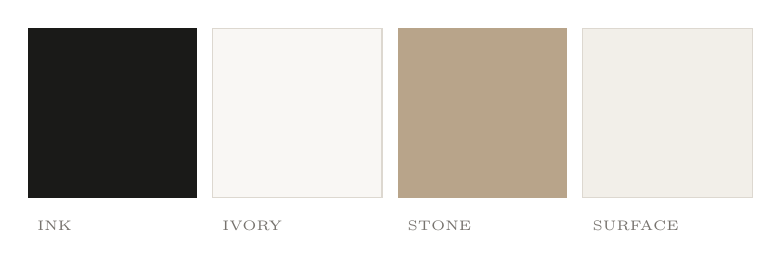
\begin{tikzpicture}
    \fill[MarkouInk] (0,0) rectangle (2.15,2.15);
    \fill[MarkouIvory,draw=MarkouLine] (2.35,0) rectangle (4.5,2.15);
    \fill[MarkouStone] (4.7,0) rectangle (6.85,2.15);
    \fill[MarkouSurface,draw=MarkouLine] (7.05,0) rectangle (9.2,2.15);
    \node[anchor=north west,text=MarkouMuted,font=\tiny] at (0,-0.18) {INK};
    \node[anchor=north west,text=MarkouMuted,font=\tiny] at (2.35,-0.18) {IVORY};
    \node[anchor=north west,text=MarkouMuted,font=\tiny] at (4.7,-0.18) {STONE};
    \node[anchor=north west,text=MarkouMuted,font=\tiny] at (7.05,-0.18) {SURFACE};
  \end{tikzpicture}
\end{minipage}\hfill
\begin{minipage}[t]{0.47\textwidth}
  \eyebrow{Typographic voice}\par\vspace{3mm}
  {\DisplayFont\fontsize{28}{29}\selectfont Material, light\\and proportion.}\par
  \vspace{3mm}
  {\fontsize{8}{11}\selectfont\bfseries\textls[180]{DETAIL / PRECISION / PLACE}}\par
  \vspace{2mm}
  {\small\color{MarkouMuted}Editorial display type creates warmth and
  distinction; a neutral sans serif keeps navigation and practical information
  direct.}
\end{minipage}

\vspace{8mm}
\begin{multicols}{2}
\feature{01 / Warm minimalism}{
Ivory and surface tones replace sterile white, while charcoal replaces absolute
black. The result has the softness of natural materials without sacrificing
contrast or clarity.}

\columnbreak
\feature{02 / Stone as a signal}{
The taupe accent is reserved for labels, rules, locations, controls and active
states. Its scarcity gives it meaning and mirrors the site's quiet confidence.}
\end{multicols}

\begin{multicols}{2}
\feature{03 / Editorial scale}{
Cormorant-led headings introduce fashion and interiors sensibility. Fluid type
scales maintain that character from mobile screens to wide desktop canvases.}

\columnbreak
\feature{04 / Image-led proof}{
Portrait, landscape and moving imagery are arranged with asymmetric pacing so
the portfolio feels curated rather than fed from a uniform catalogue grid.}
\end{multicols}

\section{Signature Experience Moments}
\subsection{A video-first opening sequence}
The homepage hero behaves as a moving material board. Multiple workshop and
finished-interior films are composed into responsive panels, with a dedicated
mobile feature selection. Poster imagery, deferred sources and playback
coordination preserve the intended first impression when bandwidth or browser
autoplay behaviour varies.

\subsection{Motion with architectural purpose}
Reveals use measured vertical travel and an expressive easing curve rather than
constant movement. Project imagery receives a slow, controlled zoom; navigation
states change with the underlying surface; and links underline progressively.
Together, these interactions indicate hierarchy and reward exploration without
competing with the work.

\subsection{Project-to-project continuity}
The experience warms internal destinations during pointer, focus and touch
intent, then carries users through a bespoke page transition. This turns a set
of static routes into a more continuous portfolio journey while preserving
native URLs, browser history and crawlability.

\begin{darkbox}
\eyebrow{Responsive media orchestration}\par\vspace{3mm}
\begin{tabularx}{\textwidth}{>{\color{MarkouStone}\bfseries}p{34mm} X}
Desktop & Multi-panel cinematic compositions create breadth and abundance.\\
Mobile & A single featured film protects legibility, memory and bandwidth.\\
Off-screen media & Intersection-based control limits unnecessary playback.\\
Background tabs & Visibility handling pauses work the visitor cannot see.\\
Fallback state & Still imagery protects the composition when video is delayed.\\
\end{tabularx}
\end{darkbox}

\section{Content Architecture}
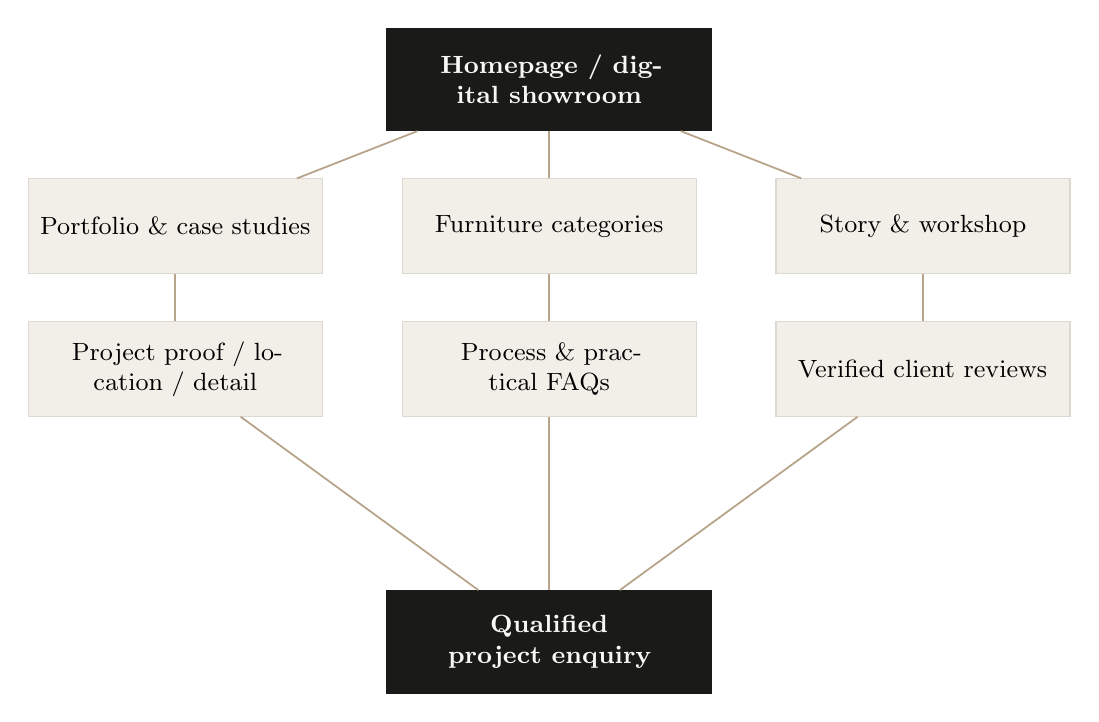
\begin{tikzpicture}[
  node distance=6mm and 8mm,
  box/.style={draw=MarkouLine,fill=MarkouSurface,minimum height=12mm,
    text width=35mm,align=center,font=\small},
  root/.style={draw=MarkouInk,fill=MarkouInk,text=MarkouIvory,
    minimum height=13mm,text width=39mm,align=center,font=\bfseries\small},
  line/.style={draw=MarkouStone,line width=.65pt}
]
\node[root] (home) {Homepage / digital showroom};
\node[box,below left=of home] (work) {Portfolio \& case studies};
\node[box,below=of home] (services) {Furniture categories};
\node[box,below right=of home] (story) {Story \& workshop};
\node[box,below=of work] (proof) {Project proof / location / detail};
\node[box,below=of services] (process) {Process \& practical FAQs};
\node[box,below=of story] (reviews) {Verified client reviews};
\node[root,below=22mm of process] (contact) {Qualified project enquiry};
\draw[line] (home) -- (work);
\draw[line] (home) -- (services);
\draw[line] (home) -- (story);
\draw[line] (work) -- (proof);
\draw[line] (services) -- (process);
\draw[line] (story) -- (reviews);
\draw[line] (proof) -- (contact);
\draw[line] (process) -- (contact);
\draw[line] (reviews) -- (contact);
\end{tikzpicture}

% ==========================================================================
% 03 — TECHNOLOGY
% ==========================================================================
\chapteropener
  {03 / Platform architecture}
  {Beauty on the surface.\\Discipline underneath.}
  {A static-first frontend, managed cloud services and focused custom
JavaScript deliver a premium experience without making the public site
dependent on a heavy application framework.}

\section{Architecture at a Glance}
\begin{center}
\begin{tikzpicture}[
  node distance=7mm,
  layer/.style={draw=MarkouLine,fill=MarkouSurface,text width=148mm,
    minimum height=17mm,align=left,inner xsep=6mm,font=\small},
  arrow/.style={->,draw=MarkouStone,line width=.8pt}
]
\node[layer] (experience) {\textbf{Experience layer}\hspace{4mm}
Semantic HTML \textbullet\ Tailwind/CSS \textbullet\ responsive media
\textbullet\ native interaction and animation modules};
\node[layer,below=of experience] (delivery) {\textbf{Delivery layer}\hspace{4mm}
Firebase Hosting \textbullet\ global CDN \textbullet\ managed HTTPS
\textbullet\ immutable asset caching \textbullet\ canonical redirects};
\node[layer,below=of delivery] (data) {\textbf{Data \& operations}\hspace{4mm}
Cloud Firestore \textbullet\ qualified leads \textbullet\ behavioural events
\textbullet\ authenticated analytical dashboard};
\node[layer,below=of data] (automation) {\textbf{Automation layer}\hspace{4mm}
Firebase Function \textbullet\ secret-managed Microsoft Graph credentials
\textbullet\ lead email delivery status};
\draw[arrow] (experience) -- (delivery);
\draw[arrow] (delivery) -- (data);
\draw[arrow] (data) -- (automation);
\end{tikzpicture}
\end{center}

\subsection{Static-first public experience}
The public site is delivered as HTML, CSS and JavaScript. This keeps the main
journey close to the browser platform: content remains directly addressable,
metadata remains visible to crawlers, and interactions can be progressively
enhanced instead of gating the entire interface behind a client-side runtime.

\subsection{Purpose-built enhancement modules}
Navigation, footer composition, animation, media behaviour, reviews, case-study
layouts, contact capture and analytics are separated into focused assets. This
reduces coupling and makes it possible to improve one experience layer without
rebuilding unrelated pages.

\subsection{A repeatable build pipeline}
The project includes scripted generation for Tailwind CSS, homepage styles,
public-page preparation, static-asset optimisation, cache-busting, sitemaps and
robots directives. Repetition is automated so production releases are less
dependent on manual edits.

\section{Lead Generation \& Operations}
\begin{tabularx}{\textwidth}{>{\color{MarkouStone}\DisplayFont\Large}p{15mm} X}
01 & \textbf{Capture.} The enquiry flow records contact details, project type,
postcode and a meaningful brief rather than collecting only an email address.\\
02 & \textbf{Persist.} Leads are written to a constrained Firestore collection
with timestamps, source and session context.\\
03 & \textbf{Notify.} A document-created cloud trigger obtains a
secret-protected Microsoft access token and sends a formatted lead notification.\\
04 & \textbf{Operate.} Authorised users can review leads, change status and
inspect acquisition and engagement data in the analytical dashboard.\\
\end{tabularx}

\vspace{5mm}
\begin{insightbox}
\eyebrow{Security boundary}\par\vspace{2mm}
\small
Public clients may create only explicitly permitted event and lead shapes.
Administrative reading, lead updates and deletion require an authenticated,
approved identity. Unknown Firestore paths are denied by default, and Microsoft
credentials are declared as managed function secrets rather than public
frontend configuration.
\end{insightbox}

\section{Measurement Designed for Decisions}
The project records first-party behavioural events with page, session, referrer
and device context. The dashboard then turns that stream into an operational
view of visits, engagement and enquiries. The intent is not surveillance; it is
to answer practical questions:

\begin{itemize}
  \item Which project and service pages create meaningful interest?
  \item Which sources bring visitors who progress toward an enquiry?
  \item Where does the browsing journey stop before contact?
  \item Which project types and locations appear most often in leads?
\end{itemize}

% ==========================================================================
% 04 — QUALITY
% ==========================================================================
\chapteropener
  {04 / Quality foundation}
  {Discoverable.\\Responsive. Responsible.}
  {Premium presentation earns attention; technical quality protects it across
devices, networks, assistive technologies and search journeys.}

\section{Search Architecture}
\begin{multicols}{2}
\small
\textbf{Descriptive page intent.} Core pages and case studies use specific
titles and descriptions around fitted wardrobes, joinery, locations and
project types. This aligns landing-page language with real client searches.

\textbf{Structured entities.} The homepage publishes organisation, furniture
store, website, webpage and FAQ data. The graph connects the brand, service
area, social profiles and frequently asked questions in machine-readable form.

\columnbreak
\textbf{Index control.} Canonical links, XML sitemaps, crawler directives and
production redirects provide a coherent URL layer for both legacy and clean
routes.

\textbf{Social presentation.} Open Graph and Twitter metadata define the title,
summary and representative imagery used when project pages are shared.
\end{multicols}

\begin{darkbox}
\begin{center}
{\DisplayFont\fontsize{27}{30}\selectfont\color{MarkouStone}London / Hertfordshire / Essex}\par
\vspace{2mm}
{\small\color{MarkouIvory}The service area is expressed consistently in
visitor-facing copy and structured business data.}
\end{center}
\end{darkbox}

\section{Performance as Art Direction}
Performance choices are part of the design because timing changes how quality
is perceived. The implementation includes:

\begin{itemize}
  \item self-hosted display and sans-serif fonts to remove avoidable
  cross-origin request chains;
  \item preload hints for critical font resources and a priority still image
  for the opening composition;
  \item deferred video sources, responsive image sets and lazy decoding for
  portfolio imagery;
  \item intent-based page warming before internal navigation;
  \item long-lived immutable caching for versioned images, fonts and video;
  \item visibility and intersection handling that prevents off-screen media
  from consuming unnecessary resources;
  \item hashed asset versions generated during optimisation to keep releases
  cache-safe.
\end{itemize}

\section{Inclusive Interaction}
\begin{tabularx}{\textwidth}{p{40mm} X}
\toprule
\eyebrow{Principle} & \eyebrow{Delivered consideration}\\
\midrule
Keyboard operation & Review controls, links and focus-driven route warming
support non-pointer interaction.\\
Motion awareness & The enhancement layer can respect reduced-motion
preferences and avoid making movement essential to comprehension.\\
Media resilience & Poster/fallback states maintain meaning when video does not
load or cannot autoplay.\\
Semantic cues & Descriptive image alternatives, labelled controls, heading
structure and explicit regions improve interpretation.\\
Responsive clarity & Mobile media selection, fluid layout and bounded
typography prevent desktop spectacle from overwhelming smaller screens.\\
\bottomrule
\end{tabularx}

\begin{insightbox}
\eyebrow{Quality principle}\par\vspace{2mm}
\small
An Awwwards-level experience is not defined by animation density. It is defined
by coherence: brand, motion, speed, content and conversion all reinforcing the
same idea without one undermining another.
\end{insightbox}

% ==========================================================================
% 05 — DELIVERY
% ==========================================================================
\chapteropener
  {05 / Delivery scope}
  {The visible finish is\\only the final layer.}
  {Behind the interface sits research, content architecture, responsive
engineering, media preparation, cloud operations, quality assurance and launch
stewardship.}

\section{Indicative Effort \& Complexity}
The table below describes the specialist effort required to recreate a platform
of this breadth and finish from a clean starting point. It is a reasoned
production estimate, not a timesheet.

\begin{tabularx}{\textwidth}{>{\bfseries}p{49mm} >{\raggedleft\arraybackslash}p{22mm} X}
\toprule
\eyebrow{Workstream} & \eyebrow{Indicative effort} & \eyebrow{Principal outputs}\\
\midrule
Discovery \& experience strategy & 18--24 hrs &
Audience intent, positioning, content model, route plan and conversion journey\\
Visual system \& responsive direction & 28--36 hrs &
Palette, typography, spacing, art direction, component states and breakpoints\\
Homepage \& core page engineering & 38--48 hrs &
Cinematic hero, responsive layouts, navigation, footer and interaction system\\
Portfolio \& case-study system & 30--40 hrs &
Project taxonomy, editorial layouts, reusable case-study enhancements and media\\
Media preparation \& performance & 20--28 hrs &
Responsive images, video behaviour, fallbacks, fonts, caching and asset versions\\
Lead capture \& cloud automation & 24--32 hrs &
Firestore model, security rules, notification function and delivery status\\
Analytics \& admin dashboard & 24--34 hrs &
Event capture, session context, authenticated reporting and lead workflow\\
SEO, accessibility \& structured data & 18--24 hrs &
Metadata, schema, sitemaps, redirects, semantic and keyboard review\\
Cross-device QA \& deployment & 22--30 hrs &
Browser testing, regression repair, build automation and Firebase release\\
\midrule
\textcolor{MarkouStone}{Total recreation range} &
\textcolor{MarkouStone}{222--296 hrs} &
\textcolor{MarkouMuted}{Approximately 5.5--7.5 specialist working weeks}\\
\bottomrule
\end{tabularx}

\vspace{4mm}
{\scriptsize\color{MarkouMuted}
Estimate assumes supplied brand content and photography, and excludes ongoing
copywriting, new photography, paid-media management and post-launch retainers.
}

\section{Delivered Platform Footprint}
\begin{center}
\metric{21}{HTML destinations}{Homepage, services, story, portfolio, policies and case studies.}
\hfill
\metric{14}{Public JS modules}{Interaction, reviews, media, analytics, contact and admin behaviour.}
\hfill
\metric{28}{Hosting mappings}{Redirect and source entries supporting clean production routing.}
\end{center}

\vspace{8mm}
\begin{center}
\metric{13}{Project videos}{Cinematic workshop and finished-space media in the public project library.}
\hfill
\metric{1}{Cloud trigger}{Automated lead notification on new Firestore documents.}
\hfill
\metric{1}{Unified system}{Brand experience, discovery, conversion and operations.}
\end{center}

\section{What the Investment Creates}
\begin{multicols}{2}
\feature{Brand equity}{
A distinctive presentation moves the studio away from commodity comparison and
toward design-led consideration.}

\feature{Qualified demand}{
Case studies, process clarity and a structured enquiry path help visitors
self-select before the studio invests consultation time.}

\columnbreak
\feature{Reusable proof}{
Each new project can become a search destination, social asset and visual proof
point inside the wider portfolio.}

\feature{Operational memory}{
Lead status and first-party interaction data create a view of what the website
is producing, not simply what it looks like.}
\end{multicols}

\pullquote{The website is both showroom and infrastructure: one earns desire,
the other makes that attention useful.}

% ==========================================================================
% 06 — CONCLUSION
% ==========================================================================
\chapteropener
  {06 / Conclusion}
  {A digital flagship\\with workshop values.}
  {Designed to age with the brand, the platform pairs expressive presentation
with a dependable path from discovery to qualified conversation.}

\section{Final Assessment}
\begin{multicols}{2}
\small
The Markou Design London platform succeeds because its creative and technical
choices share a single premise: \textbf{precision communicates care}. The warm
neutral palette, serif scale, slow image movement and editorial compositions
make the work feel considered. The case-study routes, structured metadata and
responsive assets make it discoverable. The lead and analytics systems make it
operational.

This is not a visual skin placed over a generic funnel. It is a tailored digital
environment that respects the pace and substance of bespoke joinery. Visitors
are invited to look closely, understand the process and arrive at the enquiry
form with a stronger sense of fit.

Its long-term value will come from stewardship: publishing excellent completed
projects, maintaining accurate structured data, reviewing performance evidence,
and preserving the restraint that gives the experience its character.
\end{multicols}

\vspace{5mm}
\begin{darkbox}
\eyebrow{The platform in one line}\par\vspace{4mm}
{\DisplayFont\fontsize{25}{29}\selectfont
A quiet, cinematic digital showroom that turns craftsmanship into confidence
and confidence into conversation.}
\end{darkbox}

\section{Recommended Stewardship}
\begin{enumerate}
  \item Publish each significant commission as a location-aware case study with
  a concise brief, material notes and edited photography.
  \item Review search queries, project-page engagement and lead quality
  quarterly; optimise for useful demand rather than raw traffic.
  \item Keep video edits short, muted and purposeful, with tested still
  fallbacks and mobile-specific selections.
  \item Run accessibility, broken-link, structured-data and performance checks
  as part of every meaningful release.
  \item Protect the design system: use the stone accent sparingly, maintain
  generous whitespace and let project evidence lead.
\end{enumerate}

\vfill
\begin{center}
  {\color{MarkouStone}\rule{24mm}{1pt}}\par
  \vspace{5mm}
  {\DisplayFont\fontsize{23}{27}\selectfont Markou Design London}\par
  \vspace{2mm}
  {\small\color{MarkouMuted}Digital Experience \& Client Study}\par
  \vspace{7mm}
  {\scriptsize\bfseries\textls[170]{PREPARED BY ROCK \& BLU LTD}}\par
  \vspace{2mm}
  {\scriptsize\color{MarkouMuted}July 2026}
\end{center}

\end{document}
